\vspace{-1em}
\subsection{Trust Nodes and Trust Functions}

\begin{figure}[htbp]
\centering
\begin{subfigure}{0.18\textwidth}
  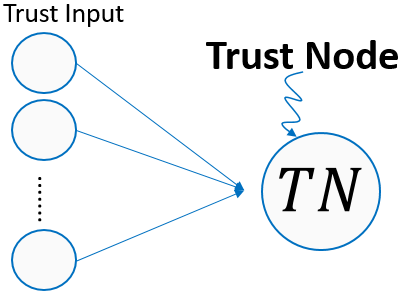
\includegraphics[width=\textwidth]{good_figs/trust_node/trustnode.png}
  \caption{Trust Node}
  \label{fig:tns}
\end{subfigure}
\hfill
\begin{subfigure}{0.30\textwidth}
  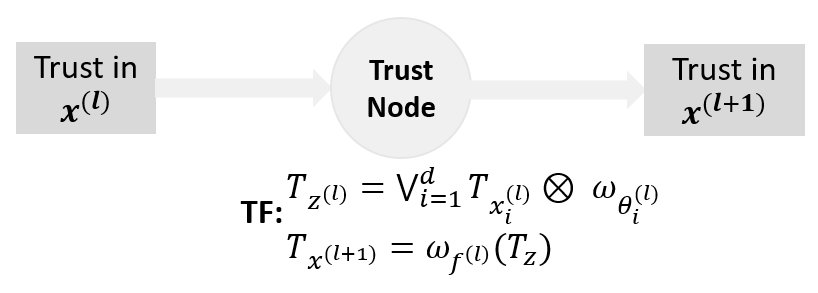
\includegraphics[width=\textwidth]{good_figs/trust_node/tnop.png}
  \caption{Trust Function operation}
  \label{fig:tnf}
\end{subfigure}
\caption{Trust Node structure and computation, mirroring the corresponding neuron (shown side by side in Appendix~\ref{app:trustnode}).}
\label{fig:trustnode}
\end{figure}

We now need to extend our discussion of \(\pf_\Theta\) from a single perceptron to larger neural networks. In order to formalize the construction of \(\pf_\Theta\), we introduce two fundamental concepts: 
the \emph{Trust Node} (\cref{fig:tns}) and the \emph{Trust Function} (\cref{fig:tnf}). These components provide the basic mechanisms for propagating trust through the structure of a neural network. 

\begin{definition}[Trust Node]
A \emph{Trust Node} is an abstract computational unit associated with a neuron in a neural network. It receives trust opinions on the neuron’s inputs and produces a trust opinion on the neuron’s output. The structure of a Trust Node mirrors that of its corresponding neuron, but its computation is defined over trust opinions using operators such as discounting and fusion.
\end{definition}

\begin{definition}[Trust Function]\label{def:trustfunc}
A \emph{Trust Function} models the transformation of trust through a Trust Node. It defines how trust opinions on the inputs of a neuron are combined to produce a trust opinion on the output. 
For a neuron that computes
\(
z^{(l)} = \sum \theta^{(l)}_i \cdot x^{(l)}_i, \quad x^{(l+1)} = \phi^{(l)}(z^{(l)}),
\)
the corresponding trust computation is given by:
\begin{equation}
T_{z^{(l)}} = \bigoplus_{i=1}^{d} T_{x_{i}^{(l)}} \otimes T_{\theta_{i}^{(l)}}, \quad
T_{x^{(l+1)}} = T_{\phi^{(l)}}(T_{z^{(l)}}),
\label{eq:layerprop}
\end{equation}
\begin{itemize}
    \item \( \otimes \) is a trust discounting operator,
    \item \(\bigoplus\) is a trust fusion operator,
    \item \( T_{\phi}^{(l)} \) is the trust-equivalent of the activation function. In this work, we set it to identity function as we use ReLU as activation function.
\end{itemize}
\end{definition}

Motivated by the structure of trust propagation in earlier sub-problems (\cref{eq:sol}), the discount operator \( \otimes \) models how trust in an input is modulated by trust in the associated parameter, while the fusion operator \( \bigoplus \) combines these trust contributions across inputs. The fusion operators should be associative or generalizable~\cite{vanderheijden2018multisourcefusionoperationssubjective} to support multiple inputs.

With these definitions in place, we integrated Trust Nodes and Trust Functions into a parallel trust reasoning framework that mirrors neural network computation. Although this was first illustrated in the perceptron case, two critical challenges remain: how to quantify the trustworthiness of model parameters learned from datasets of variable quality, and how to generalize trust propagation to deeper, more complex neural architectures. These challenges motivate the design of the Parallel Trust Assessment System (PaTAS), a scalable architecture for trust propagation in neural networks. The following section presents its design, components, and theoretical foundations.